\documentclass[11pt,a4paper]{article}

\usepackage[utf8]{inputenc}
\usepackage[T1]{fontenc}
\usepackage[polish]{babel}
\usepackage{lmodern}
\usepackage{geometry}
\usepackage{graphicx}
\usepackage{booktabs}
\usepackage{siunitx}
\usepackage{amsmath}
\usepackage{array}
\usepackage{xcolor}
\usepackage{listings}
\usepackage{hyperref}

\geometry{margin=2.5cm}
\sisetup{
  locale = PL,
  detect-all,
  group-separator = {\,},
  group-minimum-digits = 4
}
\hypersetup{
  colorlinks=true,
  linkcolor=blue!45!black,
  citecolor=blue!45!black,
  urlcolor=blue!45!black,
  pdftitle={Dyfuzyjne generowanie kodu w projekcie Diffusion-code-generation},
  pdfauthor={TODO}
}
\lstset{
  basicstyle=\ttfamily\small,
  breaklines=true,
  columns=fullflexible,
  frame=single
}

%\title{Dyfuzyjne generowanie kodu w projekcie
\title{We are better than Google - generowanie kodu z wykorzystaniem modeli dyfuzyjnych}
\author{Autorzy: Filip Lecrut, Piotr Jasiński, Weronika Wiechno}
\date{\today}

\begin{document}

\maketitle

%\tableofcontents

\section{Wprowadzenie}
\label{sec:wprowadzenie}

Generowanie kodu źródłowego jest obecnie jednym z najważniejszych kierunków rozwoju modeli generatywnych. Kod, w przeciwieństwie do zwykłego tekstu naturalnego, musi spełniać jednocześnie kilka rodzajów wymagań: powinien być poprawny składniowo, zgodny semantycznie z intencją użytkownika, możliwy do wykonania oraz spójny z kontekstem programu, w którym się znajduje. Nawet niewielki błąd, taki jak brak nawiasu, niepoprawne wcięcie, pomylenie nazwy zmiennej albo wygenerowanie instrukcji w złym miejscu, może spowodować, że cały program przestanie działać. Co istotne, błędy te mają charakter lokalny — wynikają z naruszenia krótkich, ściśle określonych wzorców składniowych — ale ich konsekwencje są globalne i mogą uniemożliwić wykonanie całego programu.

Współczesne systemy generowania kodu są najczęściej oparte na architekturze Transformer oraz mechanizmie uwagi \cite{vaswani2017attention, chen2021evaluating}. Modele te osiągają bardzo dobre wyniki, ponieważ potrafią modelować zależności pomiędzy odległymi fragmentami sekwencji. Jednak ich praktyczne wykorzystanie wiąże się z istotnymi ograniczeniami. Po pierwsze, standardowy mechanizm self-attention ma złożoność obliczeniową rosnącą kwadratowo względem długości sekwencji, czyli $\mathcal{O}(N^2)$. Oznacza to, że przetwarzanie długich plików kodu, zawierających setki lub tysiące tokenów, wymaga bardzo dużej ilości pamięci oraz mocy obliczeniowej. Po drugie, wiele modeli generuje kod autoregresyjnie, czyli token po tokenie od lewej do prawej. Taki sposób generacji powoduje, że błędna decyzja podjęta na wczesnym etapie może zostać utrwalona i wpłynąć na wszystkie kolejne fragmenty wygenerowanego kodu. Problem ten jest trudny do naprawienia bez regeneracji całości, ponieważ model nie wraca do wcześniejszych decyzji.

Problem z pamięcią i złożonością jest szczególnie istotny w przypadku większych projektów programistycznych, gdzie kod nie składa się z pojedynczej, krótkiej funkcji, lecz z wielu zależnych od siebie fragmentów. Model powinien wtedy zachować spójność nazw zmiennych, struktur sterujących, typów danych, importów, definicji funkcji oraz sposobu wykorzystania wcześniej utworzonych elementów programu.

Alternatywą dla klasycznej generacji autoregresyjnej jest maskowana dyfuzja dyskretna, w której model nie musi generować sekwencji wyłącznie od lewej do prawej \cite{austin2021structured, chang2022maskgit}. Zamiast tego proces generacji rozpoczyna się od częściowo zamaskowanej reprezentacji, a następnie model iteracyjnie przewiduje brakujące tokeny. W kolejnych krokach odsłaniane są te fragmenty, co do których model ma największą pewność. Podejście to ma szczególne znaczenie dla kodu: struktura programu często pozwala z dużą pewnością wypełnić niektóre fragmenty — np. zamknięcie bloku, słowo kluczowe \texttt{return}, nawiasy domykające — bez znajomości pozostałych. Pytaniem otwartym pozostaje jednak, jak zaprojektować architekturę modelu, który będzie w stanie efektywnie przewidywać te tokeny przy ograniczonym koszcie obliczeniowym.

W ramach niniejszego projektu proponujemy zbadanie, czy proces maskowanej dyfuzji dyskretnej może zostać zrealizowany nie przy użyciu klasycznego Transformera, lecz za pomocą architektury konwolucyjnej. Główną motywacją tego wyboru jest obserwacja, że kod źródłowy zawiera wiele silnych, lokalnych regularności. Allamanis et al. \cite{allamanis2018survey} pokazują, że kod wykazuje znacznie wyższy stopień powtarzalności niż tekst naturalny — zarówno na poziomie tokenów, jak i krótkich sekwencji. Analiza statystyczna kodu wskazuje, że znaczna część tokenów w typowym pliku źródłowym należy do niewielkiego zbioru wzorców: nawiasów, operatorów, słów kluczowych i krótkich wywołań funkcji \cite{bielik2016phog}. Sugeruje to, że duża część lokalnych decyzji generatywnych nie wymaga dostępu do całego kontekstu sekwencji.

Sieci konwolucyjne są naturalnym kandydatem do modelowania takich zależności, ponieważ analizują dane przez przesuwające się okna o stałym rozmiarze. Dzięki właściwości dzielenia wag, ta sama operacja filtrowania jest stosowana w każdym położeniu sekwencji, co pozwala na wykrywanie powtarzalnych wzorców niezależnie od ich miejsca w pliku. W porównaniu z mechanizmem uwagi, który traktuje każdą parę tokenów symetrycznie, konwolucja może dać lepsze rezultaty w kontekście lokalnym — co w przypadku kodu jest ważne.

Dodatkową zaletą sieci konwolucyjnych jest korzystniejsza skalowalność obliczeniowa. W przeciwieństwie do mechanizmu uwagi, którego koszt rośnie kwadratowo względem długości sekwencji, operacje konwolucyjne mogą być wykonywane z kosztem liniowym względem długości wejścia \cite{wu2019pay, gehring2017convolutional}.

Sama lokalność konwolucji może jednak nie wystarczyć do poprawnego generowania kodu. Programy zawierają bowiem również zależności o większym zasięgu, takie jak użycie zmiennej zdefiniowanej wiele linii wcześniej, odwołania do funkcji, zależności pomiędzy importami a późniejszym kodem czy zgodność typów. Dlatego w projekcie zastosowano architekturę, w której kolejne warstwy konwolucyjne mają wykładniczo rosnące współczynniki rozszerzenia (ang. \textit{dilation rates}), zwiększając efektywne pole recepcyjne modelu geometrycznie wraz z głębokością sieci. Inspiracją dla takiego podejścia są architektury sekwencyjne wykorzystujące rozszerzające się konwolucje, takie jak WaveNet \cite{oord2016wavenet}, oraz prace pokazujące skuteczność modeli konwolucyjnych w zadaniach sekwencyjnych \cite{bai2018empirical}.
\section{Sformułowanie problemu}
\label{sec:problem}

Dla instrukcji naturalnojęzykowej $p$, która w naszym projekcie wygenerowana jest przez LLM - model Ollamy należy wygenerować sekwencję tokenów kodu $x_0$, która odpowiada zadaniu opisanemu przez instrukcję.
W czasie treningu znany kod referencyjny jest częściowo zastępowany tokenami \texttt{[MASK]}, a model otrzymuje zadanie przewidzenia oryginalnych tokenów w pozycjach objętych maską.

Najpierw tworzona jest uszkodzona sekwencję $x_t$ oraz maska $m$.
Maska (m) określa, które tokeny zostały ukryte: wartość (m\_i=1) oznacza pozycję zamaskowaną, natomiast (m\_i=0) — pozycję pozostawioną bez zmian.

Na podstawie uszkodzonej sekwencji model przewiduje rozkład prawdopodobieństwa tokenów dla każdej pozycji.
Funkcja straty jest jednak obliczana wyłącznie dla pozycji zamaskowanych, ponieważ to właśnie ich odtworzenia model ma się nauczyć:


\begin{equation}
\label{eq:ce}
\mathcal{L}_{CE}
= -\frac{1}{|M|}\sum_{i\in M}\log p_\theta(x_{0,i}\mid x_t,p,t),
\end{equation}

gdzie (M) jest zbiorem zamaskowanych pozycji, a (|M|) oznacza liczbę tych pozycji.
Wyrażenie z sumą oznacza prawdopodobieństwo, jakie model przypisał prawidłowemu tokenowi (x\_{0,i}) na podstawie uszkodzonej sekwencji (x\_t), kontekstu (p) oraz poziomu zaszumienia (t).

\section{Zbiór danych i przygotowanie danych}
\label{sec:dane}

Na potrzeby treningu modelu utworzono własny, syntetyczny zbiór danych zawierający polecenia programistyczne oraz odpowiadające im rozwiązania w języku Python. Dane zostały wygenerowane przy użyciu lokalnie uruchamianego dużego modelu językowego za pośrednictwem środowiska Ollama.

Proces tworzenia zbioru przebiegał w trzech etapach. W pierwszej kolejności wygenerowano 500 tematów związanych z programowaniem. Następnie dla każdego tematu przygotowano po 15 różnych poleceń programistycznych. Ostatnim etapem było wygenerowanie wielu rozwiązań dla każdego polecenia.

Każdy rekord zbioru zawiera temat zadania, treść instrukcji oraz wygenerowany kod. Dodatkowo przechowywane są identyfikatory tematu i instrukcji, numer wariantu rozwiązania oraz informacje związane z kontrolą poprawności kodu.

\begin{table}[htbp]
\centering
\caption{Podsumowanie dostępnych plików danych.}
\label{tab:dane-podsumowanie}
\begin{tabular}{lS}
\toprule
\textbf{Artefakt} & {\textbf{Liczba wierszy}} \\
\midrule
\texttt{data/dataset.csv} & 107554 \\
\texttt{data/topics.csv} & 500  \\
\texttt{data/instructions.csv} & 7500  \\
\texttt{data/dataset.csv} & 106262\\
\bottomrule
\end{tabular}
\end{table}



Przed przekazaniem danych do modelu tekst instrukcji oraz kod źródłowy zostały zamienione na sekwencje tokenów. Przy podziale zbioru na część treningową i walidacyjną uwzględniono powiązania między wariantami. Wszystkie rozwiązania wygenerowane dla tej samej instrukcji znajdowały się w tej samej części zbioru. Zapobiega to sytuacji, w której model jest trenowany na jednym wariancie rozwiązania, a następnie oceniany na bardzo podobnym wariancie tego samego zadania.


%
%Plik \texttt{data/dataset.csv} zawiera kolumny \texttt{topic\_id}, \texttt{instruction\_id}, \texttt{topic}, \texttt{instruction}, \texttt{code}, \texttt{valid}, \texttt{variant\_idx}, \texttt{id}, \texttt{code\_file}, \texttt{compile\_valid}, \texttt{validation\_error} oraz \texttt{runtime\_valid}. Do budowy cache aktywnie używane są co najmniej \texttt{instruction} i \texttt{code}, a filtry mogą wykorzystywać \texttt{valid} i \texttt{compile\_valid}. Liczebności pokazane w tabelach~\ref{tab:dane-podsumowanie} i~\ref{tab:dane-jakosc} pochodzą z materiałów dowodowych i bezpośredniego zliczenia plików CSV.
%
%Funkcja \texttt{ensure\_tokenized\_cache()} w \texttt{src/tokenized\_dataset.py} wykonuje filtrowanie, tokenizację oraz zapis macierzy \texttt{.npy}. Filtr \texttt{DATASET\_REQUIRE\_VALID} ogranicza dane do wierszy z \texttt{valid=True}, a \texttt{DATASET\_COMPILE\_FILTER} może wymagać \texttt{compile\_valid=True} albo tylko wykluczać jawne \texttt{False}. W aktualnych metadanych cache występuje tryb \texttt{exclude\_false}.
%
%\input{tables/cache_summary}
%
%Podział na trening i walidację realizuje \texttt{make\_train\_val\_indices()}. Funkcja może używać \texttt{group\_ids}, dzięki czemu warianty tej samej znormalizowanej instrukcji nie powinny trafiać jednocześnie do części treningowej i walidacyjnej. Nie znaleziono zapisanego \texttt{TRAIN\_RESULT\_JSON}, dlatego faktycznych liczebności podziału dla konkretnego przebiegu nie można potwierdzić.

\section{Tokenizacja }
\label{sec:tokenizacja}

Tokenizację obsługuje \texttt{Qwen/Qwen2.5-Coder-7B}. W preprocessinu dopisywany jest token \texttt{[CODE\_EOS]} na końcu każdego kodu oraz zapewniane jest istnienie tokenów \texttt{pad} i \texttt{mask}. Instrukcje są normalizowane przez zamianę na małe litery i redukcję białych znaków, natomiast kod jest tokenizowany bez takiej normalizacji.



\section{Metoda maskowania}
\label{sec:maskowanie}

Podczas uczenia część tokenów w sekwencji kodu jest zastępowana specjalnym tokenem maskującym. Zadaniem modelu jest następnie odtworzenie ukrytych elementów na podstawie widocznej części kodu, opisu zadania oraz informacji o poziomie zaszumienia.

Poziom maskowania nie jest stały. Dla każdej sekwencji losowany jest udział tokenów, które mają zostać ukryte. Stosowana jest mieszanina kilku zakresów maskowania: niskiego, średniego, wysokiego oraz pełnego. Dzięki temu model uczy się zarówno uzupełniania pojedynczych brakujących fragmentów, jak i generowania większych części programu przy bardzo ograniczonym dostępie do oryginalnego kodu. Próbki o niskim poziomie maskowania wspierają naukę lokalnej składni, natomiast próbki o wysokim poziomie maskowania zmuszają model do silniejszego wykorzystywania treści polecenia.

Maskowaniu podlegają wyłącznie właściwe tokeny kodu. Tokeny techniczne, takie jak znaczniki początku i końca sekwencji oraz tokeny dopełniające, są chronione i pozostają niezmienione.

Ukrywane pozycje mogą być wybierane na kilka sposobów. W maskowaniu niezależnym tokeny są wybierane losowo w całej sekwencji. Maskowanie blokowe usuwa spójne fragmenty kodu, co przypomina sytuację, w której brakuje całego wyrażenia lub instrukcji. W innych wariantach widoczny pozostaje początek programu, a maskowana jest jego dalsza część, albo usuwany jest końcowy fragment sekwencji. Możliwe jest również pełne zamaskowanie wszystkich dostępnych tokenów kodu. Zastosowanie różnych wariantów ma przygotować model do rozwiązywania zróżnicowanych zadań rekonstrukcji i generowania.

Przy bardzo wysokim poziomie maskowania ograniczane są warianty pozostawiające długi, uporządkowany fragment kodu. Zapobiega to sytuacji, w której model opiera swoje przewidywania głównie na widocznym początku lub końcu programu zamiast na treści polecenia.

Podczas walidacji wykorzystywane są również stałe, deterministycznie generowane maski. Oznacza to, że te same przykłady są oceniane przy użyciu tych samych ukrytych pozycji w kolejnych epokach. Pozwala to rzetelnie porównywać zmiany jakości modelu podczas treningu i ogranicza wpływ losowości na uzyskiwane wyniki.


\section{Architektura modelu}
\label{sec:architektura_modelu}

Zastosowany model jest warunkowym modelem dyfuzyjnym przeznaczonym do generowania kodu źródłowego na podstawie opisu zadania (Schemat całej architektury przedstawiliśmy na Rysunku~\ref{fig:model-architecture}). Jego wejście składa się z dwóch części: instrukcji tekstowej określającej wymagane działanie programu oraz częściowo zamaskowanej sekwencji kodu. Model otrzymuje również informację o aktualnym poziomie zaszumienia, czyli o tym, jaka część kodu została ukryta.

Tokeny instrukcji i kodu są najpierw przekształcane na reprezentacje wektorowe. Do każdej reprezentacji dodawana jest informacja o pozycji tokenu w sekwencji, dzięki czemu model może rozróżniać kolejność elementów programu. Reprezentacje instrukcji i kodu są następnie łączone w jedną sekwencję. Tokeny dopełniające, stosowane jedynie w celu wyrównania długości przykładów, są zerowane, aby nie wpływały na dalsze obliczenia.

%\begin{figure}[htbp]
\centering
\setlength{\fboxsep}{8pt}
\fbox{\begin{minipage}{0.88\linewidth}
\centering
\texttt{.env} i zmienne środowiskowe\\
$\downarrow$\\
\texttt{src/train.py::main} $\rightarrow$ \texttt{Config} $\rightarrow$ \texttt{DiffCoderTrainer}\\
$\downarrow$\\
\texttt{data/dataset.csv}\\
$\downarrow$\\
\texttt{ensure\_tokenized\_cache} i \texttt{TokenizedMemmapDataset}\\
$\downarrow$\\
\texttt{MixtureMaskSampler} $\rightarrow$ \texttt{CodeCorruptor}\\
$\downarrow$\\
\texttt{LocalConvDiffCoder.forward}\\
$\downarrow$\\
\texttt{cross entropy} / opcjonalnie \texttt{aligned\_multi\_reference\_cross\_entropy} / opcjonalnie \texttt{CalculateLoss}\\
$\downarrow$\\
\texttt{AdamW} + \texttt{LambdaLR} + \texttt{Trainer}\\
$\downarrow$\\
walidacja, checkpointy, generowanie diagnostyczne
\end{minipage}}
\caption{Aktywna ścieżka treningu zrekonstruowana z \texttt{src/train.py}, \texttt{src/tokenized\_dataset.py}, \texttt{src/diffusion/masking.py} i \texttt{src/diffusion/model.py}.}
\label{fig:architektura}
\end{figure}



\begin{figure}[htbp]
\centering
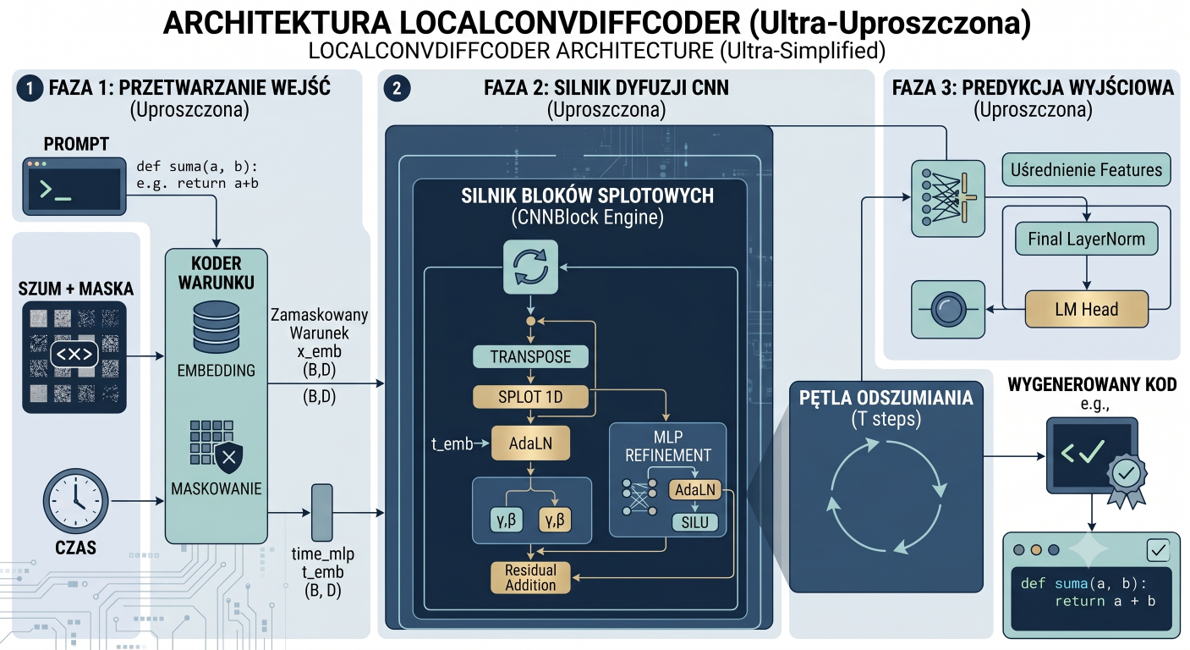
\includegraphics[width=0.9\linewidth]{figures/architecture}
\caption{Schemat architektury modelu dyfuzyjnego z jednowymiarowymi blokami splotowymi.}
\label{fig:model-architecture}
\end{figure}

Główną część modelu stanowi stos bloków splotowych. Sploty jednowymiarowe analizują lokalne zależności między sąsiednimi tokenami, takie jak struktura wyrażeń, argumenty funkcji czy kolejne elementy instrukcji. W kolejnych blokach zwiększane są rozmiar jądra i dylacja, co pozwala obejmować coraz większe fragmenty sekwencji bez konieczności znacznego zwiększania liczby warstw. Dzięki temu model może jednocześnie uwzględniać lokalną składnię oraz zależności występujące między bardziej odległymi częściami programu.

Każdy blok wykorzystuje połączenia rezydualne, normalizację, warstwę nieliniową oraz dropout. Połączenia rezydualne ułatwiają przepływ informacji i stabilizują uczenie głębszej sieci. Normalizacja jest dodatkowo modyfikowana na podstawie poziomu zaszumienia, dzięki czemu sposób przetwarzania sekwencji zależy od liczby ukrytych tokenów. Model może więc inaczej zachowywać się podczas uzupełniania niewielkiego fragmentu kodu, a inaczej podczas odtwarzania prawie całego programu.

Reprezentacje otrzymane w kolejnych blokach są łączone, a następnie wybierana jest część odpowiadająca tokenom kodu. Końcowa warstwa przekształca reprezentację każdej pozycji na rozkład prawdopodobieństwa obejmujący całe słownictwo tokenizatora. Na tej podstawie model przewiduje, jakie tokeny powinny znaleźć się w zamaskowanych miejscach.

Rozmiar reprezentacji, liczba bloków splotowych, poziom dylacji i wartość dropout są parametrami konfiguracyjnymi. Mogą być zatem dostosowywane do wielkości zbioru danych, dostępnych zasobów obliczeniowych oraz wymaganej pojemności modelu.


\section{Uzasadnienie alternatywnej architektury - użycie bloków splotowych zamiast transformera}
\label{sec:uzasadnienie_architektury}

Współczesne systemy generowania kodu są najczęściej oparte na architekturze Transformer oraz mechanizmie uwagi \cite{vaswani2017attention, chen2021evaluating}. Modele te osiągają bardzo dobre wyniki, ponieważ potrafią modelować zależności pomiędzy odległymi fragmentami sekwencji. Jednak ich praktyczne wykorzystanie wiąże się z istotnymi ograniczeniami. Po pierwsze, standardowy mechanizm self-attention ma złożoność obliczeniową rosnącą kwadratowo względem długości sekwencji, czyli $\mathcal{O}(N^2)$. Oznacza to, że przetwarzanie długich plików kodu, zawierających setki lub tysiące tokenów, wymaga bardzo dużej ilości pamięci oraz mocy obliczeniowej. Po drugie, wiele modeli generuje kod autoregresyjnie, czyli token po tokenie od lewej do prawej. Taki sposób generacji powoduje, że błędna decyzja podjęta na wczesnym etapie może zostać utrwalona i wpłynąć na wszystkie kolejne fragmenty wygenerowanego kodu. Problem ten jest trudny do naprawienia bez regeneracji całości, ponieważ model nie wraca do wcześniejszych decyzji.

Problem z pamięcią i złożonością jest szczególnie istotny w przypadku większych projektów programistycznych, gdzie kod nie składa się z pojedynczej, krótkiej funkcji, lecz z wielu zależnych od siebie fragmentów. Model powinien wtedy zachować spójność nazw zmiennych, struktur sterujących, typów danych, importów, definicji funkcji oraz sposobu wykorzystania wcześniej utworzonych elementów programu.

Alternatywą dla klasycznej generacji autoregresyjnej jest maskowana dyfuzja dyskretna, w której model nie musi generować sekwencji wyłącznie od lewej do prawej \cite{austin2021structured, chang2022maskgit}. Zamiast tego proces generacji rozpoczyna się od częściowo zamaskowanej reprezentacji, a następnie model iteracyjnie przewiduje brakujące tokeny. W kolejnych krokach odsłaniane są te fragmenty, co do których model ma największą pewność. Podejście to ma szczególne znaczenie dla kodu: struktura programu często pozwala z dużą pewnością wypełnić niektóre fragmenty — np. zamknięcie bloku, słowo kluczowe \texttt{return}, nawiasy domykające — bez znajomości pozostałych. Pytaniem otwartym pozostaje jednak, jak zaprojektować architekturę modelu, który będzie w stanie efektywnie przewidywać te tokeny przy ograniczonym koszcie obliczeniowym.

W ramach niniejszego projektu proponujemy zbadanie, czy proces maskowanej dyfuzji dyskretnej może zostać zrealizowany nie przy użyciu klasycznego Transformera, lecz za pomocą architektury konwolucyjnej. Główną motywacją tego wyboru jest obserwacja, że kod źródłowy zawiera wiele silnych, lokalnych regularności. Allamanis et al. \cite{allamanis2018survey} pokazują, że kod wykazuje znacznie wyższy stopień powtarzalności niż tekst naturalny — zarówno na poziomie tokenów, jak i krótkich sekwencji. Analiza statystyczna kodu wskazuje, że znaczna część tokenów w typowym pliku źródłowym należy do niewielkiego zbioru wzorców: nawiasów, operatorów, słów kluczowych i krótkich wywołań funkcji \cite{bielik2016phog}. Sugeruje to, że duża część lokalnych decyzń generatywnych nie wymaga dostępu do całego kontekstu sekwencji.

Sieci konwolucyjne są naturalnym kandydatem do modelowania takich zależności, ponieważ analizują dane przez przesuwające się okna o stałym rozmiarze. Dzięki właściwości dzielenia wag, ta sama operacja filtrowania jest stosowana w każdym położeniu sekwencji, co pozwala na wykrywanie powtarzalnych wzorców niezależnie od ich miejsca w pliku. W porównaniu z mechanizmem uwagi, który traktuje każdą parę tokenów symetrycznie, konwolucja może dać lepsze rezultaty w kontekście lokalnym — co w przypadku kodu jest ważne.

Dodatkową zaletą sieci konwolucyjnych jest korzystniejsza skalowalność obliczeniowa. W przeciwieństwie do mechanizmu uwagi, którego koszt rośnie kwadratowo względem długości sekwencji, operacje konwolucyjne mogą być wykonywane z kosztem liniowym względem długości wejścia \cite{wu2019pay, gehring2017convolutional}.

Sama lokalność konwolucji może jednak nie wystarczyć do poprawnego generowania kodu. Programy zawierają bowiem również zależności o większym zasięgu, takie jak użycie zmiennej zdefiniowanej wiele linii wcześniej, odwołania do funkcji, zależności pomiędzy importami a późniejszym kodem czy zgodność typów. Dlatego w projekcie zastosowano architekturę, w której kolejne warstwy konwolucyjne mają wykładniczo rosnące współczynniki rozszerzenia (ang. \textit{dilation rates}), zwiększając efektywne pole recepcyjne modelu geometrycznie wraz z głębokością sieci. Inspiracją dla takiego podejścia są architektury sekwencyjne wykorzystujące rozszerzające się konwolucje, takie jak WaveNet \cite{oord2016wavenet}, oraz prace pokazujące skuteczność modeli konwolucyjnych w zadaniach sekwencyjnych \cite{bai2018empirical}.

\section{Funkcja straty}
\label{sec:strata}

Podstawowym celem uczenia jest poprawne odtworzenie tokenów usuniętych podczas maskowania. Model przewiduje rozkład prawdopodobieństwa dla każdej zamaskowanej pozycji, a następnie porównuje go z prawidłowym tokenem pochodzącym z oryginalnego programu. Podstawową funkcją straty jest entropia krzyżowa, obliczana wyłącznie dla pozycji, które zostały ukryte. Tokeny pozostawione bez zmian nie uczestniczą bezpośrednio w obliczaniu tej części straty.

Każdy błędnie przewidziany token wpływa na wynik zgodnie z prawdopodobieństwem przypisanym poprawnej odpowiedzi. Projekt umożliwia również uczenie z wieloma poprawnymi rozwiązaniami tego samego zadania. Jeżeli dla jednej instrukcji dostępnych jest kilka równoważnych programów, przewidywanie modelu może być porównywane z referencją najlepiej zgodną z widoczną częścią kodu. Dzięki temu model nie jest niepotrzebnie karany za wygenerowanie poprawnego rozwiązania, które różni się od jednego arbitralnie wybranego programu referencyjnego.

Strata strukturalna wykorzystuje abstrakcyjne drzewo składniowe programu. Reprezentacja generowanego kodu jest wówczas porównywana z reprezentacją sekwencji elementów drzewa składniowego. Do ich dopasowania wykorzystywany jest algorytm Soft-DTW, który pozwala porównywać sekwencje o różnych długościach i uwzględnia możliwe przesunięcia pomiędzy elementami.

Porównywana jest też strata dla właściwego opisu zadania oraz dla opisu pochodzącego z innego przykładu. Model jest karany, jeżeli nie wykorzystuje poprawnej instrukcji wyraźnie lepiej niż instrukcji niedopasowanej. Ma to ograniczyć generowanie kodu opartego wyłącznie na częstości wzorców występujących w zbiorze danych.


\section{Proces treningu}
\label{sec:trening}

W każdej iteracji treningowej pobierana jest partia przykładów zawierających opisy zadań oraz odpowiadające im programy. Dla każdej sekwencji losowany jest poziom maskowania, po czym wybrane tokeny kodu są zastępowane maskami.

Model przewiduje tokeny dla zamaskowanych pozycji, a uzyskane predykcje są porównywane z oryginalnym kodem. Na tej podstawie obliczana jest funkcja straty, a parametry modelu są aktualizowane.




\section{Walidacja i metryki}
\label{sec:walidacja}

Pierwsza część walidacji odwzorowuje warunki treningowe. Poziom i sposób maskowania są losowane z tego samego rozkładu co podczas uczenia. Uzyskana strata pokazuje więc, jak model radzi sobie przeciętnie z zadaniami podobnymi do tych, które obserwuje w trakcie treningu.

Druga część wykorzystuje ustalone poziomy maskowania: \num{0.25}, \num{0.50}, \num{0.75}, \num{0.95} oraz \num{1.00}. Dla każdego poziomu generowane są deterministyczne maski, dzięki czemu te same tokeny pozostają ukryte w kolejnych epokach. Umożliwia to bezpośrednie porównywanie jakości modelu w czasie, bez zakłóceń wynikających z losowego wyboru pozycji.

Kolejna diagnostyka sprawdza, czy model rzeczywiście korzysta z opisu zadania. Dla tego samego zamaskowanego kodu porównywane są predykcje otrzymane z poprawną instrukcją oraz z instrukcją przypisaną do innego przykładu. Jeżeli właściwa instrukcja prowadzi do niższej straty, oznacza to, że model wykorzystuje jej treść podczas przewidywania kodu. Niewielka różnica może natomiast sugerować, że model zbyt mocno opiera się na widocznych fragmentach programu lub na ogólnych wzorcach występujących w zbiorze danych.

Oprócz straty oceniane są właściwości wygenerowanych programów. Poprawność składniowa określa, jaki odsetek wyników może zostać przetworzony do postaci abstrakcyjnego drzewa składniowego języka Python. Osobna miara sprawdza, czy kod może zostać skompilowany bez wystąpienia błędu składniowego.

Do porównania wygenerowanego programu z rozwiązaniem referencyjnym wykorzystywana jest również odległość Levenshteina. Określa ona minimalną liczbę operacji wstawienia, usunięcia lub zamiany znaku potrzebnych do przekształcenia jednego tekstu w drugi. Wersja znormalizowana dzieli uzyskaną wartość przez długość dłuższego tekstu, dzięki czemu możliwe jest porównywanie programów o różnej długości. Niższa wartość oznacza większe podobieństwo do rozwiązania referencyjnego.



\section{Inferencja i generowanie}
\label{sec:inferencja}

Podczas inferencji model generuje program na podstawie samego opisu zadania. Proces rozpoczyna się od sekwencji, w której wszystkie pozycje przeznaczone na kod są wypełnione tokenem maskującym. Model wielokrotnie analizuje tę sekwencję i stopniowo zastępuje maski przewidywanymi tokenami.

W każdym kroku model wyznacza rozkład prawdopodobieństwa dla wszystkich nadal nieustalonych pozycji. Na jego podstawie wybierane są najbardziej prawdopodobne tokeny oraz określana jest pewność poszczególnych przewidywań. Liczba pozostających masek jest stopniowo zmniejszana, aż do uzyskania kompletnej sekwencji kodu.

W strategii podstawowej tokeny o najwyższej pewności są utrwalane wcześniej, natomiast pozycje o niższej pewności pozostają zamaskowane i są ponownie przewidywane w kolejnych krokach. Umożliwia to stopniowe przechodzenie od ogólnego zarysu programu do bardziej szczegółowych decyzji dotyczących jego składni.

Iteracyjny charakter procesu odróżnia zastosowane podejście od modeli autoregresyjnych, które generują kod kolejno od lewej do prawej. Model dyfuzyjny może modyfikować wiele pozycji jednocześnie oraz ponownie oceniać wcześniejsze decyzje na podstawie aktualnego stanu całej sekwencji.




\section{Wyniki eksperymentów}
\label{sec:wyniki}

Do oceny wydajności i zachowania modelu wybrano eksperyment z najlepszymi artefaktami kodowymi, którego logi i dane wykresów zostały wyeksportowane do katalogu \texttt{best\_results/}. Analiza opiera się na przebiegu treningu trwającym ponad \num{22800} kroków.

W tabeli~\ref{tab:metryki-comet} przedstawiono wybrane końcowe metryki walidacyjne zarejestrowane w platformie Comet ML dla kroku \num{40299}. Dla dokładniejszego zbadania zachowania modelu w czasie treningu przeanalizowano dodatkowe charakterystyki opisane poniżej.

\input{tables/comet_metrics}

\subsection{Zachowanie straty przy różnych poziomach szumu}

Model dyfuzyjny w trakcie treningu uczy się rekonstrukcji tokenów przy różnym natężeniu szumu (różnych proporcjach maskowania kodu). Rysunek~\ref{fig:val-loss-masking} przedstawia przebieg straty walidacyjnej (\textit{Validation Loss}) dla czterech dyskretnych poziomów maskowania: \num{25}\%, \num{50}\%, \num{75}\% oraz \num{95}\%, a także ogólną średnią stratę walidacyjną.

\begin{figure}[htbp]
\centering
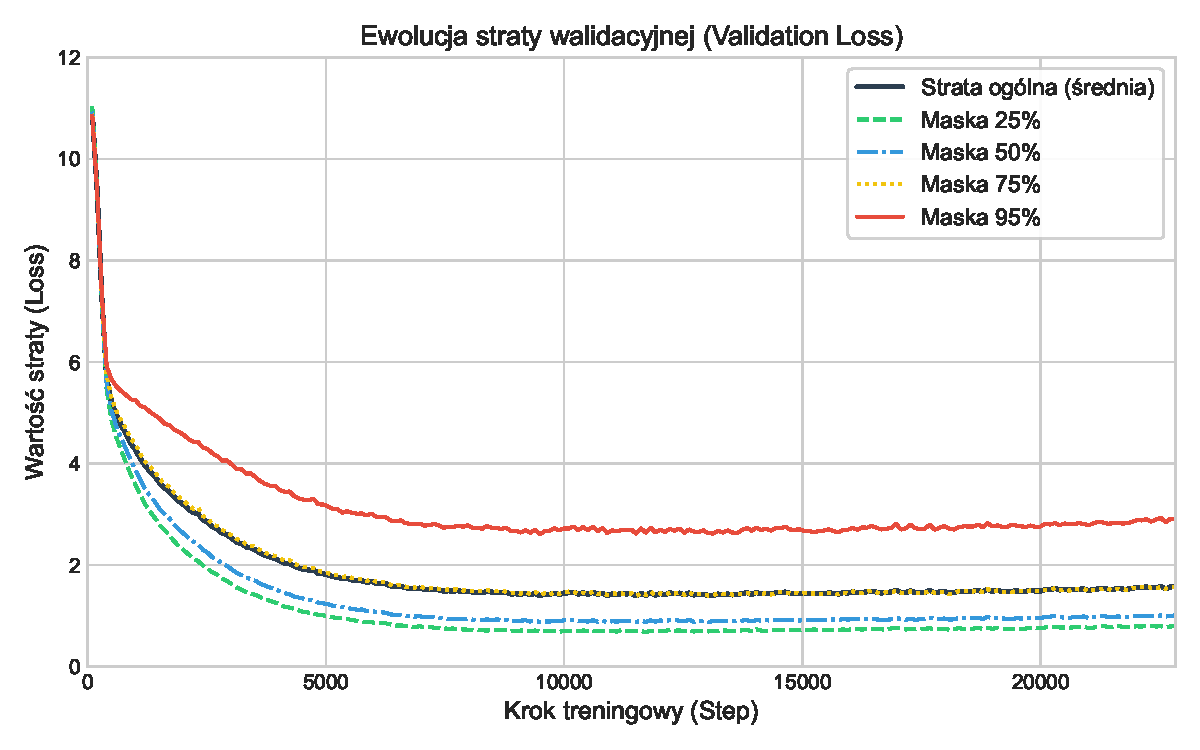
\includegraphics[width=0.85\linewidth]{figures/val_loss_masking}
\caption{Przebieg straty walidacyjnej w zależności od stopnia zamaskowania kodu (proporcji szumu) w trakcie treningu.}
\label{fig:val-loss-masking}
\end{figure}

Z wykresu wynika, że strata dla maskowania \num{25}\% (\textit{zielona linia przerywana}) jest najniższa i spada najszybciej, osiągając wartość końcową ok. \num{0.68}. Jest to zgodne z intuicją, ponieważ model, mając dostęp do \num{75}\% oryginalnego kodu (wysoki kontekst), ma znacznie ułatwione zadanie rekonstrukcji pozostałych tokenów. Z kolei strata dla maskowania \num{95}\% (\textit{czerwona linia ciągła}) reprezentuje sytuację ekstremalną, w której model musi zrekonstruować niemal cały kod wyłącznie na podstawie instrukcji naturalnojęzykowej i nielicznych tokenów pomocniczych. Ta strata również wykazuje tendencję spadkową w trakcie treningu (z poziomu ok. \num{10.8} do ok. \num{2.6}), co dowodzi, że model uczy się generowania kodu od podstaw. Wszystkie krzywe charakteryzują się gładką zbieżnością bez wyraźnych oznak przeuczenia (overfittingu) w badanym zakresie kroków, co potwierdza stabilność procesu treningowego.

\subsection{Wrażliwość modelu na instrukcje (Prompt Shuffling)}

Kluczową cechą warunkowego modelu generowania kodu jest jego sterowalność za pomocą instrukcji w języku naturalnym (promptu). Aby sprawdzić, czy model rzeczywiście bierze pod uwagę treść instrukcji, czy jedynie uczy się bezwarunkowego rozkładu kodu, zastosowano procedurę zaburzania kontekstu (\textit{Prompt Shuffling}). Polega ona na losowym przetasowaniu tokenów promptu podczas walidacji przy pełnym zamaskowaniu kodu (\num{100}\%).

Rysunek~\ref{fig:val-prompt-shuffle} przedstawia porównanie straty walidacyjnej przy oryginalnym promptcie (\textit{Original Prompt}) oraz przy zaburzonym promptcie (\textit{Shuffled Prompt}), a także różnicę między nimi (\textit{Delta}).

\begin{figure}[htbp]
\centering
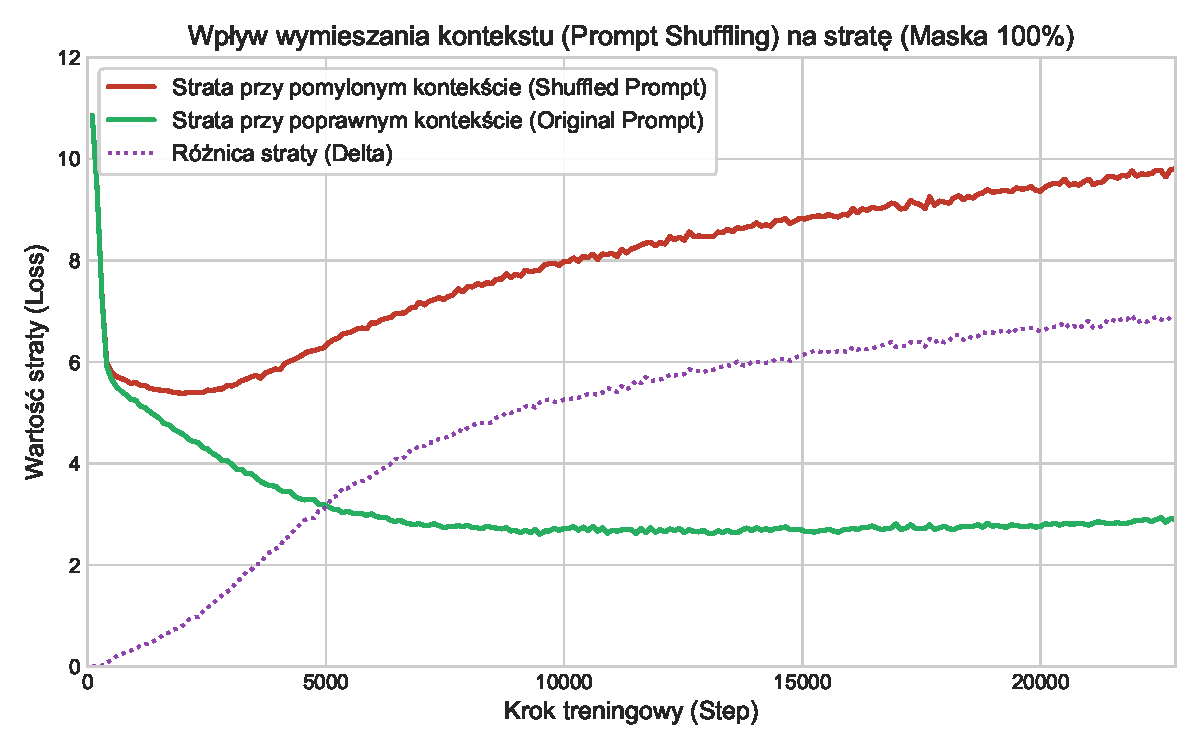
\includegraphics[width=0.85\linewidth]{figures/val_prompt_shuffle}
\caption{Wpływ przetasowania tokenów instrukcji (Prompt Shuffling) na wartość straty walidacyjnej przy maskowaniu \num{100}\%.}
\label{fig:val-prompt-shuffle}
\end{figure}

Analiza wykresu wskazuje na wyraźne różnice w zachowaniu modelu w zależności od poprawności instrukcji warunkującej. Strata przy zaburzonym promptcie (\textit{czerwona linia}) pozostaje na bardzo wysokim poziomie w trakcie całego treningu, spadając jedynie nieznacznie z ok. \num{10.8} do ok. \num{5.4}. W tym samym czasie strata przy poprawnym promptcie (\textit{zielona linia}) zbiega do wartości ok. \num{1.4}. W konsekwencji różnica straty (\textit{fioletowa linia przerywana}) rośnie w miarę postępu treningu, osiągając ostatecznie wartość ok. \num{6.9}. Wynik ten jednoznacznie potwierdza, że model rozwija silną zależność od struktury i semantyki promptu. Gdy instrukcja jest pozbawiona sensu wskutek przetasowania tokenów, zdolność modelu do poprawnej rekonstrukcji kodu drastycznie maleje.

\subsection{Dynamika procesu generowania (Remasking Dynamics)}

Podczas inferencji model generuje kod w sposób iteracyjny, wykorzystując procedurę ponownego maskowania tokenów o niskiej pewności (remaskowanie). Rysunek~\ref{fig:val-generation-remasking} przedstawia średnią liczbę remaskowanych tokenów na krok w zależności od zaawansowania treningu.

\begin{figure}[htbp]
\centering
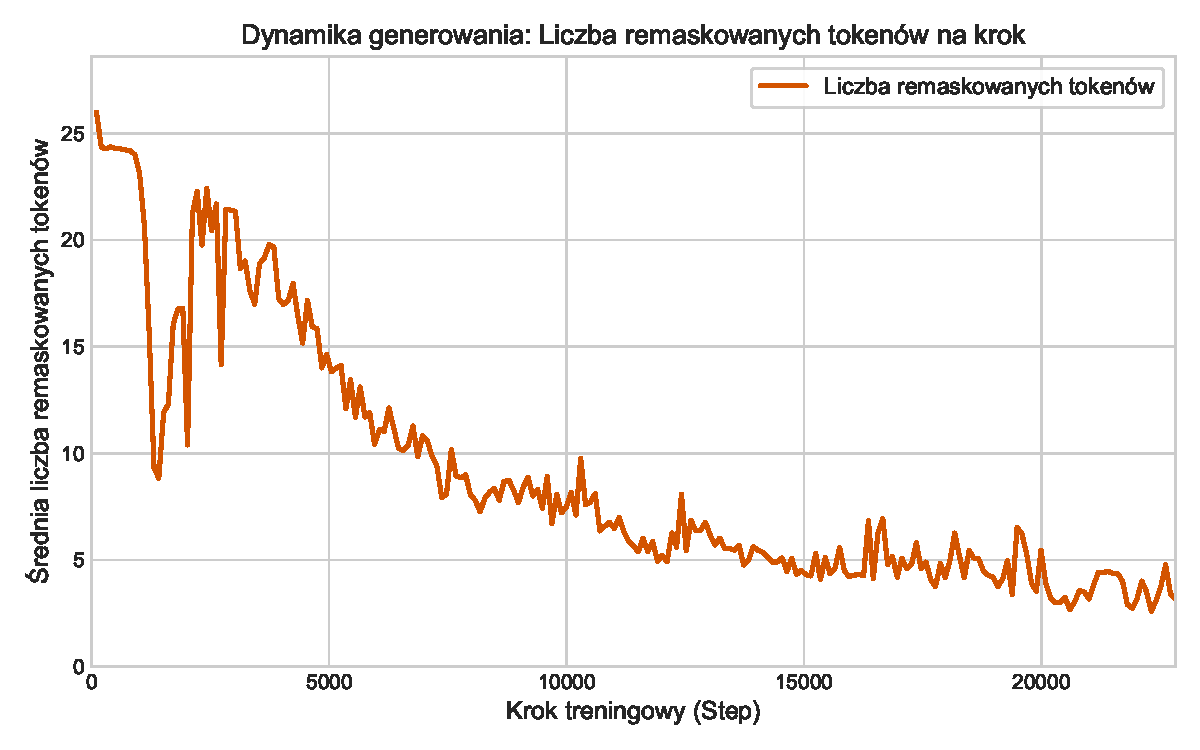
\includegraphics[width=0.85\linewidth]{figures/val_generation_remasking}
\caption{Średnia liczba tokenów oznaczanych jako niepewne i remaskowanych w pojedynczym kroku inferencji generatywnej w trakcie treningu.}
\label{fig:val-generation-remasking}
\end{figure}

Przedstawiony wykres ilustruje ewolucję dynamiki remaskowania w czasie. Na początku procesu treningowego model remaskuje średnio ok. \num{26} tokenów na krok, co świadczy o dużej niepewności w generowanych sekwencjach. W miarę postępu treningu średnia ta systematycznie spada, osiągając na końcu wartość ok. \num{2.6} tokena na krok. Spadek ten dowodzi, że model w kolejnych epokach generuje kod w sposób bardziej spójny i zdecydowany, produkując tokeny o wysokim prawdopodobieństwie już w pierwszych krokach generacji, co bezpośrednio skraca i stabilizuje iteracyjny proces próbkowania.

\section{Analiza jakościowa generowanych przykładów}
\label{sec:przyklady}

Aby lepiej zrozumieć, jak nasz model radzi sobie z pisaniem kodu, przeanalizowaliśmy kilka konkretnych przykładów, które wygenerował. Podzieliliśmy je na udane (czyli takie, które działają i nie mają błędów) oraz nieudane (które zawierają błędy składniowe lub logiczne). Pełne kody tych przykładów znajdują się w dodatkach na końcu raportu.

\subsection{Przykłady poprawnych generacji (Dodatek A)}

Model pokazał, że potrafi napisać działający kod na podstawie prostego polecenia w języku angielskim. Oto dwa ciekawe przykłady:

\begin{enumerate}
  \item \textbf{Porównywanie dat} (Próbka \texttt{text-sample-13836 (1).txt}): 
  Ten kod (znajdziesz go na Listingu~\ref{lst:text-sample-13836-1} w Dodatku~\ref{app:kody-kompilowalne}) poprawnie porównuje dwie daty wpisane jako tekst. Model sam zaimportował moduł \texttt{datetime}, napisał funkcję \texttt{compare\_dates} i dodał blok \texttt{try-except}, który chroni program przed crashowaniem, jeśli ktoś poda zły format daty. Co ciekawe, model dopisał też na końcu testy (w bloku \texttt{if \_\_name\_\_ == '\_\_main\_\_':}), sprawdzając poprawność kodu dla różnych danych. Pokazuje to, że model nauczył się nie tylko samej funkcji, ale też sposobu jej testowania.
  
  \item \textbf{Szukanie środkowego elementu} (Próbka \texttt{text-sample-14340 (2).txt}):
  Kod na Listingu~\ref{lst:text-sample-14340-2} w Dodatku~\ref{app:kody-kompilowalne} realizuje zadanie szukania środka listy. Model dobrze zrozumiał warunek: jeśli lista ma parzystą długość, zwraca element o jeden wcześniej niż rzeczywisty środek, a w przeciwnym razie zwraca dokładny środek. Użył do tego dzielenia całkowitego (\texttt{n // 2}), co chroni przed błędami z indeksami ułamkowymi. Tutaj również model dodał testowe listy na końcu, by sprawdzić działanie kodu.
\end{enumerate}

\subsection{Przykłady generacji z błędami (Dodatek B)}

Analiza błędów pozwala nam zobaczyć, z czym model radzi sobie najgorzej. Szczegółowe zestawienie problemów opisaliśmy w Dodatku~\ref{app:bledy-generacji}. Oto najczęstsze z nich:

\begin{enumerate}
  \item \textbf{Niezbalansowane nawiasy} (Próbka \texttt{text-sample-504 (1).txt}):
  Na Listingu~\ref{lst:text-sample-504-1} w Dodatku~\ref{app:bledy-generacji} widać kod, w którym model zapisał samotny nawias zamykający w nagłówku funkcji. Model czasami gubi się w nawiasach przy dłuższych linijkach, bo nie zna reguł gramatycznych Pythona, a jedynie przewiduje kolejne tokeny na podstawie statystyki.
  
  \item \textbf{Niezgodność nazw} (Próbka \texttt{text-sample-16966 (3).txt}):
  W kodzie z Listingu~\ref{lst:text-sample-16966-3} w Dodatku~\ref{app:bledy-generacji} pojawia się błąd \texttt{NameError}. Funkcja przyjmuje parametry o nazwach \texttt{date\_str} i \texttt{date2\_str2}, ale w środku funkcji model używa zmiennych \texttt{date\_str1} oraz \texttt{date\_str2}. Pokazuje to, że model potrafi stworzyć poprawną strukturę (np. pętle czy warunki), ale nie pamięta dokładnie nazw zmiennych, które sam zdefiniował chwilę wcześniej.
  
  \item \textbf{Przypisanie do liczby} (Próbka \texttt{text-sample-11008 (2).txt}):
  Na Listingu~\ref{lst:text-sample-11008-2} w Dodatku~\ref{app:bledy-generacji} model napisał instrukcję typu \texttt{26 = ...}. To poważny błąd składniowy – nie można przypisać wartości do stałej liczbowej. Świadczy to o tym, że model nie rozumie logicznej roli znaku równości, a jedynie układa znaki tak, jak widział je w zbiorze treningowym.
\end{enumerate}
\section{Podsumowanie}
\label{sec:podsumowanie}

TODO


\bibliographystyle{plain}
\bibliography{bibliografia}

\clearpage
\appendix
\section{Wygenerowane programy przechodzące kontrolę kompilacji}
\label{app:kody-kompilowalne}

Ten appendix zawiera wygenerowane i kompilujące się bloki kodu (wygenerowane od zera - z sekcji \texttt{GENERATED:}), które zostały zapisane na potrzeby logowania postępów treningu (dlatego są to próbki dla tych samych instrukcji).

Ten test potwierdza poprawność składniową, lecz nie stanowi dowodu zgodności z poleceniem. Z 49 bloków oznaczonych jako \texttt{SUCCESS} zamieszczono 31 unikalnych programów. Próbki o tym samym znormalizowanym drzewie AST oraz te, które były np. samymi zerami pominięto.


\subsection{Próbka text-sample-13836 (1).txt}
\label{sec:lst:text-sample-13836-1}
\textbf{Instrukcja (Prompt):} \textit{Implement an optimized function named \texttt{compare\_dates} that accepts two date strings (in \texttt{YYYY-MM-DD} format) and returns the earlier date as a datetime object. Ensure the function is efficient and handles potential \texttt{ValueError} exceptions gracefully.}

\lstinputlisting[language=Python,caption={Pełny wygenerowany kod dla próbki text-sample-13836 (1).txt; liczba linii: \num{28}},label={lst:text-sample-13836-1}]{generated/compiled_samples/text-sample-13836-1.py}


\subsection{Próbka text-sample-14038 (3).txt}
\label{sec:lst:text-sample-14038-3}
\textbf{Instrukcja (Prompt):} \textit{Implement an optimized function named \texttt{compare\_dates} that accepts two date strings (in \texttt{YYYY-MM-DD} format) and returns the earlier date as a datetime object. Ensure the function is efficient and handles potential \texttt{ValueError} exceptions gracefully.}

\lstinputlisting[language=Python,caption={Pełny wygenerowany kod dla próbki text-sample-14038 (3).txt; liczba linii: \num{28}},label={lst:text-sample-14038-3}]{generated/compiled_samples/text-sample-14038-3.py}


\subsection{Próbka text-sample-14340 (2).txt}
\label{sec:lst:text-sample-14340-2}
\textbf{Instrukcja (Prompt):} \textit{Implement a function \texttt{find\_middle\_element} that takes a list of floats and returns the element exactly in the center. If the list has an even number of elements, return the element at the lower middle index.}

\lstinputlisting[language=Python,caption={Pełny wygenerowany kod dla próbki text-sample-14340 (2).txt; liczba linii: \num{18}},label={lst:text-sample-14340-2}]{generated/compiled_samples/text-sample-14340-2.py}


\subsection{Próbka text-sample-14542 (3).txt}
\label{sec:lst:text-sample-14542-3}
\textbf{Instrukcja (Prompt):} \textit{Implement a function \texttt{find\_middle\_element} that takes a list of floats and returns the element exactly in the center. If the list has an even number of elements, return the element at the lower middle index.}

\lstinputlisting[language=Python,caption={Pełny wygenerowany kod dla próbki text-sample-14542 (3).txt; liczba linii: \num{18}},label={lst:text-sample-14542-3}]{generated/compiled_samples/text-sample-14542-3.py}


\subsection{Próbka text-sample-14644 (1).txt}
\label{sec:lst:text-sample-14644-1}
\textbf{Instrukcja (Prompt):} \textit{Implement an optimized function named \texttt{compare\_dates} that accepts two date strings (in \texttt{YYYY-MM-DD} format) and returns the earlier date as a datetime object. Ensure the function is efficient and handles potential \texttt{ValueError} exceptions gracefully.}

\lstinputlisting[language=Python,caption={Pełny wygenerowany kod dla próbki text-sample-14644 (1).txt; liczba linii: \num{28}},label={lst:text-sample-14644-1}]{generated/compiled_samples/text-sample-14644-1.py}


\subsection{Próbka text-sample-14644 (3).txt}
\label{sec:lst:text-sample-14644-3}
\textbf{Instrukcja (Prompt):} \textit{Implement a function \texttt{find\_middle\_element} that takes a list of floats and returns the element exactly in the center. If the list has an even number of elements, return the element at the lower middle index.}

\lstinputlisting[language=Python,caption={Pełny wygenerowany kod dla próbki text-sample-14644 (3).txt; liczba linii: \num{18}},label={lst:text-sample-14644-3}]{generated/compiled_samples/text-sample-14644-3.py}


\subsection{Próbka text-sample-14744 (3).txt}
\label{sec:lst:text-sample-14744-3}
\textbf{Instrukcja (Prompt):} \textit{Implement a function \texttt{find\_middle\_element} that takes a list of floats and returns the element exactly in the center. If the list has an even number of elements, return the element at the lower middle index.}

\lstinputlisting[language=Python,caption={Pełny wygenerowany kod dla próbki text-sample-14744 (3).txt; liczba linii: \num{18}},label={lst:text-sample-14744-3}]{generated/compiled_samples/text-sample-14744-3.py}


\subsection{Próbka text-sample-14946 (2).txt}
\label{sec:lst:text-sample-14946-2}
\textbf{Instrukcja (Prompt):} \textit{Implement a function \texttt{find\_middle\_element} that takes a list of floats and returns the element exactly in the center. If the list has an even number of elements, return the element at the lower middle index.}

\lstinputlisting[language=Python,caption={Pełny wygenerowany kod dla próbki text-sample-14946 (2).txt; liczba linii: \num{18}},label={lst:text-sample-14946-2}]{generated/compiled_samples/text-sample-14946-2.py}


\subsection{Próbka text-sample-15048 (1).txt}
\label{sec:lst:text-sample-15048-1}
\textbf{Instrukcja (Prompt):} \textit{Implement a function \texttt{find\_middle\_element} that takes a list of floats and returns the element exactly in the center. If the list has an even number of elements, return the element at the lower middle index.}

\lstinputlisting[language=Python,caption={Pełny wygenerowany kod dla próbki text-sample-15048 (1).txt; liczba linii: \num{18}},label={lst:text-sample-15048-1}]{generated/compiled_samples/text-sample-15048-1.py}

% Pominięto zduplikowaną próbkę text-sample-15350-3.py; ten sam AST co text-sample-14644-1.py.

\subsection{Próbka text-sample-15956 (1).txt}
\label{sec:lst:text-sample-15956-1}
\textbf{Instrukcja (Prompt):} \textit{Implement a function \texttt{find\_middle\_element} that takes a list of floats and returns the element exactly in the center. If the list has an even number of elements, return the element at the lower middle index.}

\lstinputlisting[language=Python,caption={Pełny wygenerowany kod dla próbki text-sample-15956 (1).txt; liczba linii: \num{18}},label={lst:text-sample-15956-1}]{generated/compiled_samples/text-sample-15956-1.py}

% Pominięto zduplikowane próbki text-sample-15956-3.py i text-sample-16058-1.py; ten sam AST co text-sample-14644-1.py.

\subsection{Próbka text-sample-16360 (2).txt}
\label{sec:lst:text-sample-16360-2}
\textbf{Instrukcja (Prompt):} \textit{Implement a function \texttt{find\_middle\_element} that takes a list of floats and returns the element exactly in the center. If the list has an even number of elements, return the element at the lower middle index.}

\lstinputlisting[language=Python,caption={Pełny wygenerowany kod dla próbki text-sample-16360 (2).txt; liczba linii: \num{19}},label={lst:text-sample-16360-2}]{generated/compiled_samples/text-sample-16360-2.py}

% Pominięto zduplikowane próbki text-sample-16462-3.py, text-sample-16664-1.py i text-sample-17774-2.py; ten sam AST co text-sample-14340-2.py.
% Pominięto zduplikowane próbki text-sample-16562-2.py, text-sample-16764-3.py, text-sample-16866-3.py, text-sample-17168-3.py i text-sample-19694-3.py; ten sam AST co text-sample-14644-1.py.

\subsection{Próbka text-sample-17472 (1).txt}
\label{sec:lst:text-sample-17472-1}
\textbf{Instrukcja (Prompt):} \textit{Implement a function \texttt{find\_middle\_element} that takes a list of floats and returns the element exactly in the center. If the list has an even number of elements, return the element at the lower middle index.}

\lstinputlisting[language=Python,caption={Pełny wygenerowany kod dla próbki text-sample-17472 (1).txt; liczba linii: \num{18}},label={lst:text-sample-17472-1}]{generated/compiled_samples/text-sample-17472-1.py}


\subsection{Próbka text-sample-17976 (2).txt}
\label{sec:lst:text-sample-17976-2}
\textbf{Instrukcja (Prompt):} \textit{Implement a function \texttt{find\_middle\_element} that takes a list of floats and returns the element exactly in the center. If the list has an even number of elements, return the element at the lower middle index.}

\lstinputlisting[language=Python,caption={Pełny wygenerowany kod dla próbki text-sample-17976 (2).txt; liczba linii: \num{18}},label={lst:text-sample-17976-2}]{generated/compiled_samples/text-sample-17976-2.py}


\subsection{Próbka text-sample-18280 (3).txt}
\label{sec:lst:text-sample-18280-3}
\textbf{Instrukcja (Prompt):} \textit{Implement an optimized function named \texttt{compare\_dates} that accepts two date strings (in \texttt{YYYY-MM-DD} format) and returns the earlier date as a datetime object. Ensure the function is efficient and handles potential \texttt{ValueError} exceptions gracefully.}

\lstinputlisting[language=Python,caption={Pełny wygenerowany kod dla próbki text-sample-18280 (3).txt; liczba linii: \num{28}},label={lst:text-sample-18280-3}]{generated/compiled_samples/text-sample-18280-3.py}


\subsection{Próbka text-sample-18684 (3).txt}
\label{sec:lst:text-sample-18684-3}
\textbf{Instrukcja (Prompt):} \textit{Implement a function \texttt{find\_middle\_element} that takes a list of floats and returns the element exactly in the center. If the list has an even number of elements, return the element at the lower middle index.}

\lstinputlisting[language=Python,caption={Pełny wygenerowany kod dla próbki text-sample-18684 (3).txt; liczba linii: \num{18}},label={lst:text-sample-18684-3}]{generated/compiled_samples/text-sample-18684-3.py}


\subsection{Próbka text-sample-19188 (1).txt}
\label{sec:lst:text-sample-19188-1}
\textbf{Instrukcja (Prompt):} \textit{Implement a function \texttt{find\_middle\_element} that takes a list of floats and returns the element exactly in the center. If the list has an even number of elements, return the element at the lower middle index.}

\lstinputlisting[language=Python,caption={Pełny wygenerowany kod dla próbki text-sample-19188 (1).txt; liczba linii: \num{18}},label={lst:text-sample-19188-1}]{generated/compiled_samples/text-sample-19188-1.py}


\subsection{Próbka text-sample-19694 (1).txt}
\label{sec:lst:text-sample-19694-1}
\textbf{Instrukcja (Prompt):} \textit{Implement a function \texttt{find\_middle\_element} that takes a list of floats and returns the element exactly in the center. If the list has an even number of elements, return the element at the lower middle index.}

\lstinputlisting[language=Python,caption={Pełny wygenerowany kod dla próbki text-sample-19694 (1).txt; liczba linii: \num{18}},label={lst:text-sample-19694-1}]{generated/compiled_samples/text-sample-19694-1.py}


\subsection{Próbka text-sample-19794 (1).txt}
\label{sec:lst:text-sample-19794-1}
\textbf{Instrukcja (Prompt):} \textit{Implement an optimized function named \texttt{compare\_dates} that accepts two date strings (in \texttt{YYYY-MM-DD} format) and returns the earlier date as a datetime object. Ensure the function is efficient and handles potential \texttt{ValueError} exceptions gracefully.}

\lstinputlisting[language=Python,caption={Pełny wygenerowany kod dla próbki text-sample-19794 (1).txt; liczba linii: \num{28}},label={lst:text-sample-19794-1}]{generated/compiled_samples/text-sample-19794-1.py}


\subsection{Próbka text-sample-19794 (3).txt}
\label{sec:lst:text-sample-19794-3}
\textbf{Instrukcja (Prompt):} \textit{Implement a function \texttt{find\_middle\_element} that takes a list of floats and returns the element exactly in the center. If the list has an even number of elements, return the element at the lower middle index.}

\lstinputlisting[language=Python,caption={Pełny wygenerowany kod dla próbki text-sample-19794 (3).txt; liczba linii: \num{18}},label={lst:text-sample-19794-3}]{generated/compiled_samples/text-sample-19794-3.py}


\subsection{Próbka text-sample-19896 (3).txt}
\label{sec:lst:text-sample-19896-3}
\textbf{Instrukcja (Prompt):} \textit{Implement an optimized function named \texttt{compare\_dates} that accepts two date strings (in \texttt{YYYY-MM-DD} format) and returns the earlier date as a datetime object. Ensure the function is efficient and handles potential \texttt{ValueError} exceptions gracefully.}

\lstinputlisting[language=Python,caption={Pełny wygenerowany kod dla próbki text-sample-19896 (3).txt; liczba linii: \num{28}},label={lst:text-sample-19896-3}]{generated/compiled_samples/text-sample-19896-3.py}


\subsection{Próbka text-sample-20098 (1).txt}
\label{sec:lst:text-sample-20098-1}
\textbf{Instrukcja (Prompt):} \textit{Implement a function \texttt{find\_middle\_element} that takes a list of floats and returns the element exactly in the center. If the list has an even number of elements, return the element at the lower middle index.}

\lstinputlisting[language=Python,caption={Pełny wygenerowany kod dla próbki text-sample-20098 (1).txt; liczba linii: \num{18}},label={lst:text-sample-20098-1}]{generated/compiled_samples/text-sample-20098-1.py}

% Pominięto zduplikowaną próbkę text-sample-20098-3.py; ten sam AST co text-sample-18280-3.py.

\subsection{Próbka text-sample-20198 (3).txt}
\label{sec:lst:text-sample-20198-3}
\textbf{Instrukcja (Prompt):} \textit{Implement a function \texttt{find\_middle\_element} that takes a list of floats and returns the element exactly in the center. If the list has an even number of elements, return the element at the lower middle index.}

\lstinputlisting[language=Python,caption={Pełny wygenerowany kod dla próbki text-sample-20198 (3).txt; liczba linii: \num{18}},label={lst:text-sample-20198-3}]{generated/compiled_samples/text-sample-20198-3.py}


\subsection{Próbka text-sample-20300 (1).txt}
\label{sec:lst:text-sample-20300-1}
\textbf{Instrukcja (Prompt):} \textit{Implement an optimized function named \texttt{compare\_dates} that accepts two date strings (in \texttt{YYYY-MM-DD} format) and returns the earlier date as a datetime object. Ensure the function is efficient and handles potential \texttt{ValueError} exceptions gracefully.}

\lstinputlisting[language=Python,caption={Pełny wygenerowany kod dla próbki text-sample-20300 (1).txt; liczba linii: \num{28}},label={lst:text-sample-20300-1}]{generated/compiled_samples/text-sample-20300-1.py}

% Pominięto zduplikowaną próbkę text-sample-20300-2.py; ten sam AST co text-sample-14340-2.py.

\subsection{Próbka text-sample-20400 (3).txt}
\label{sec:lst:text-sample-20400-3}
\textbf{Instrukcja (Prompt):} \textit{Implement a function \texttt{find\_middle\_element} that takes a list of floats and returns the element exactly in the center. If the list has an even number of elements, return the element at the lower middle index.}

\lstinputlisting[language=Python,caption={Pełny wygenerowany kod dla próbki text-sample-20400 (3).txt; liczba linii: \num{18}},label={lst:text-sample-20400-3}]{generated/compiled_samples/text-sample-20400-3.py}

% Pominięto zduplikowaną próbkę text-sample-20602-1.py; ten sam AST co text-sample-19188-1.py.
% Pominięto zduplikowaną próbkę text-sample-20602-3.py; ten sam AST co text-sample-19794-1.py.

\subsection{Próbka text-sample-20804 (1).txt}
\label{sec:lst:text-sample-20804-1}
\textbf{Instrukcja (Prompt):} \textit{Implement a function \texttt{find\_middle\_element} that takes a list of floats and returns the element exactly in the center. If the list has an even number of elements, return the element at the lower middle index.}

\lstinputlisting[language=Python,caption={Pełny wygenerowany kod dla próbki text-sample-20804 (1).txt; liczba linii: \num{18}},label={lst:text-sample-20804-1}]{generated/compiled_samples/text-sample-20804-1.py}


\subsection{Próbka text-sample-20906 (2).txt}
\label{sec:lst:text-sample-20906-2}
\textbf{Instrukcja (Prompt):} \textit{Implement a function \texttt{find\_middle\_element} that takes a list of floats and returns the element exactly in the center. If the list has an even number of elements, return the element at the lower middle index.}

\lstinputlisting[language=Python,caption={Pełny wygenerowany kod dla próbki text-sample-20906 (2).txt; liczba linii: \num{18}},label={lst:text-sample-20906-2}]{generated/compiled_samples/text-sample-20906-2.py}


\subsection{Próbka text-sample-21410 (2).txt}
\label{sec:lst:text-sample-21410-2}
\textbf{Instrukcja (Prompt):} \textit{Implement a function \texttt{find\_middle\_element} that takes a list of floats and returns the element exactly in the center. If the list has an even number of elements, return the element at the lower middle index.}

\lstinputlisting[language=Python,caption={Pełny wygenerowany kod dla próbki text-sample-21410 (2).txt; liczba linii: \num{18}},label={lst:text-sample-21410-2}]{generated/compiled_samples/text-sample-21410-2.py}


\subsection{Próbka text-sample-21612 (1).txt}
\label{sec:lst:text-sample-21612-1}
\textbf{Instrukcja (Prompt):} \textit{Implement a function \texttt{find\_middle\_element} that takes a list of floats and returns the element exactly in the center. If the list has an even number of elements, return the element at the lower middle index.}

\lstinputlisting[language=Python,caption={Pełny wygenerowany kod dla próbki text-sample-21612 (1).txt; liczba linii: \num{18}},label={lst:text-sample-21612-1}]{generated/compiled_samples/text-sample-21612-1.py}


\subsection{Próbka text-sample-21714 (2).txt}
\label{sec:lst:text-sample-21714-2}
\textbf{Instrukcja (Prompt):} \textit{Implement a function \texttt{find\_middle\_element} that takes a list of floats and returns the element exactly in the center. If the list has an even number of elements, return the element at the lower middle index.}

\lstinputlisting[language=Python,caption={Pełny wygenerowany kod dla próbki text-sample-21714 (2).txt; liczba linii: \num{18}},label={lst:text-sample-21714-2}]{generated/compiled_samples/text-sample-21714-2.py}

% Pominięto zduplikowaną próbkę text-sample-21814-3.py; ten sam AST co text-sample-21714-2.py.
% Pominięto zduplikowaną próbkę text-sample-22118-2.py; ten sam AST co text-sample-20300-1.py.

\subsection{Próbka text-sample-22218 (3).txt}
\label{sec:lst:text-sample-22218-3}
\textbf{Instrukcja (Prompt):} \textit{Implement a function \texttt{find\_middle\_element} that takes a list of floats and returns the element exactly in the center. If the list has an even number of elements, return the element at the lower middle index.}

\lstinputlisting[language=Python,caption={Pełny wygenerowany kod dla próbki text-sample-22218 (3).txt; liczba linii: \num{18}},label={lst:text-sample-22218-3}]{generated/compiled_samples/text-sample-22218-3.py}

% Pominięto zduplikowaną próbkę text-sample-22320-3.py; ten sam AST co text-sample-14644-1.py.

\subsection{Próbka text-sample-22420 (2).txt}
\label{sec:lst:text-sample-22420-2}
\textbf{Instrukcja (Prompt):} \textit{Implement an optimized function named \texttt{compare\_dates} that accepts two date strings (in \texttt{YYYY-MM-DD} format) and returns the earlier date as a datetime object. Ensure the function is efficient and handles potential \texttt{ValueError} exceptions gracefully.}

\lstinputlisting[language=Python,caption={Pełny wygenerowany kod dla próbki text-sample-22420 (2).txt; liczba linii: \num{28}},label={lst:text-sample-22420-2}]{generated/compiled_samples/text-sample-22420-2.py}

\section{Najczęstsze błędy w nieudanych generacjach}
\label{app:bledy-generacji}

Do klasyfikacji błędów wykorzystano plik \texttt{text-samples/compilation\_summary.txt}, który wygenerowano za pomocą skryptu \texttt{text-samples/check\_compile.py}. W analizie uwzględniono tylko pozycje oznaczone jako \texttt{FAILED}. Próbki pominięte przez skrypt, np. zawierające wyłącznie zera, nie zostały uznane za błędy kompilacji.

W tabeli~\ref{tab:generation-bugs} przedstawiono liczbę błędów należących do poszczególnych kategorii oraz opis ich typowych objawów. Komunikaty parsera są zwykle krótkie i nie zawsze dokładnie wskazują przyczynę problemu. Z tego powodu w tabeli~\ref{tab:generation-examples} zamieszczono również podsumowanie przykładowych próbek.

\input{tables/generation_compilation_bugs}

\input{tables/generation_compilation_examples}

Przykłady pokazują, że błędy nie ograniczają się do prostych literówek. W wielu przypadkach model nie zachowuje poprawnej struktury programu. Może na przykład wygenerować nawias zamykający bez nawiasu otwierającego, połączyć fragment definicji funkcji z jej wywołaniem, nie zamknąć napisu albo utworzyć wcięty blok bez poprawnego nagłówka.

Osobną grupę stanowią programy, które są poprawne składniowo, ale zawierają błędy w nazwach zmiennych. Przykład z pliku \texttt{text-sample-16966 (3).txt} przedstawia funkcję, której ciało używa nazw innych niż nazwy podane w jej parametrach.

Poniżej przedstawiono pełne kody wygenerowane przez model (sekcje \texttt{GENERATED:}) dla każdej z reprezentatywnych próbek błędów wymienionych w tabeli~\ref{tab:generation-examples} wraz z instrukcją (promptem), który model otrzymał jako warunek generacji.


\subsection{Próbka text-sample-504 (1).txt -- Niezbalansowane nawiasy lub klamry}
\label{sec:lst:text-sample-504-1}
\textbf{Instrukcja (Prompt):} \textit{Implement an optimized function named \texttt{compare\_dates} that accepts two date strings (in \texttt{YYYY-MM-DD} format) and returns the earlier date as a datetime object. Ensure the function is efficient and handles potential \texttt{ValueError} exceptions gracefully.}

\lstinputlisting[language=Python,caption={Pełny wygenerowany kod dla próbki text-sample-504 (1).txt (Niezbalansowane nawiasy lub klamry); liczba linii: \num{33}},label={lst:text-sample-504-1}]{generated/failed_samples/text-sample-504_1.py}

\subsection{Próbka text-sample-806 (2).txt -- Ogólne błędy składni}
\label{sec:lst:text-sample-806-2}
\textbf{Instrukcja (Prompt):} \textit{Implement a function \texttt{find\_middle\_element} that takes a list of floats and returns the element exactly in the center. If the list has an even number of elements, return the element at the lower middle index.}

\lstinputlisting[language=Python,caption={Pełny wygenerowany kod dla próbki text-sample-806 (2).txt (Ogólne błędy składni); liczba linii: \num{2}},label={lst:text-sample-806-2}]{generated/failed_samples/text-sample-806_2.py}

\subsection{Próbka text-sample-1816 (1).txt -- Niedomknięte literały tekstowe}
\label{sec:lst:text-sample-1816-1}
\textbf{Instrukcja (Prompt):} \textit{Implement a function \texttt{find\_middle\_element} that takes a list of floats and returns the element exactly in the center. If the list has an even number of elements, return the element at the lower middle index.}

\lstinputlisting[language=Python,caption={Pełny wygenerowany kod dla próbki text-sample-1816 (1).txt (Niedomknięte literały tekstowe); liczba linii: \num{24}},label={lst:text-sample-1816-1}]{generated/failed_samples/text-sample-1816_1.py}

\subsection{Próbka text-sample-402 (1).txt -- Błędy wcięć i bloków}
\label{sec:lst:text-sample-402-1}
\textbf{Instrukcja (Prompt):} \textit{Implement a function \texttt{find\_middle\_element} that takes a list of floats and returns the element exactly in the center. If the list has an even number of elements, return the element at the lower middle index.}

\lstinputlisting[language=Python,caption={Pełny wygenerowany kod dla próbki text-sample-402 (1).txt (Błędy wcięć i bloków); liczba linii: \num{15}},label={lst:text-sample-402-1}]{generated/failed_samples/text-sample-402_1.py}

\subsection{Próbka text-sample-5756 (2).txt -- Błędy literałów f-string}
\label{sec:lst:text-sample-5756-2}
\textbf{Instrukcja (Prompt):} \textit{Implement an optimized class named \texttt{TimeConverter} with methods to convert between hours, minutes, and seconds, ensuring all conversion logic is mathematically sound and efficient.}

\lstinputlisting[language=Python,caption={Pełny wygenerowany kod dla próbki text-sample-5756 (2).txt (Błędy literałów f-string); liczba linii: \num{35}},label={lst:text-sample-5756-2}]{generated/failed_samples/text-sample-5756_2.py}

\subsection{Próbka text-sample-16966 (3).txt -- Niezdefiniowane nazwy}
\label{sec:lst:text-sample-16966-3}
\textbf{Instrukcja (Prompt):} \textit{Implement an optimized function named \texttt{compare\_dates} that accepts two date strings (in \texttt{YYYY-MM-DD} format) and returns the earlier date as a datetime object. Ensure the function is efficient and handles potential \texttt{ValueError} exceptions gracefully.}

\lstinputlisting[language=Python,caption={Pełny wygenerowany kod dla próbki text-sample-16966 (3).txt (Niezdefiniowane nazwy); liczba linii: \num{29}},label={lst:text-sample-16966-3}]{generated/failed_samples/text-sample-16966_3.py}

\subsection{Próbka text-sample-1008 (3).txt -- Niepoprawne literały liczbowe}
\label{sec:lst:text-sample-1008-3}
\textbf{Instrukcja (Prompt):} \textit{Implement an optimized function named \texttt{compare\_dates} that accepts two date strings (in \texttt{YYYY-MM-DD} format) and returns the earlier date as a datetime object. Ensure the function is efficient and handles potential \texttt{ValueError} exceptions gracefully.}

\lstinputlisting[language=Python,caption={Pełny wygenerowany kod dla próbki text-sample-1008 (3).txt (Niepoprawne literały liczbowe); liczba linii: \num{6}},label={lst:text-sample-1008-3}]{generated/failed_samples/text-sample-1008_3.py}

\subsection{Próbka text-sample-11008 (2).txt -- Przypisanie do literału}
\label{sec:lst:text-sample-11008-2}
\textbf{Instrukcja (Prompt):} \textit{Implement an optimized class named \texttt{TimeConverter} with methods to convert between hours, minutes, and seconds, ensuring all conversion logic is mathematically sound and efficient.}

\lstinputlisting[language=Python,caption={Pełny wygenerowany kod dla próbki text-sample-11008 (2).txt (Przypisanie do literału); liczba linii: \num{32}},label={lst:text-sample-11008-2}]{generated/failed_samples/text-sample-11008_2.py}

\subsection{Próbka text-sample-2018 (3).txt -- Niepoprawna definicja parametrów funkcji}
\label{sec:lst:text-sample-2018-3}
\textbf{Instrukcja (Prompt):} \textit{Implement an optimized class named \texttt{TimeConverter} with methods to convert between hours, minutes, and seconds, ensuring all conversion logic is mathematically sound and efficient.}

\lstinputlisting[language=Python,caption={Pełny wygenerowany kod dla próbki text-sample-2018 (3).txt (Niepoprawna definicja parametrów funkcji); liczba linii: \num{3}},label={lst:text-sample-2018-3}]{generated/failed_samples/text-sample-2018_3.py}

\subsection{Próbka text-sample-18482 (3).txt -- Niepoprawne użycie wyrażenia z gwiazdką}
\label{sec:lst:text-sample-18482-3}
\textbf{Instrukcja (Prompt):} \textit{Implement an optimized class named \texttt{TimeConverter} with methods to convert between hours, minutes, and seconds, ensuring all conversion logic is mathematically sound and efficient.}

\lstinputlisting[language=Python,caption={Pełny wygenerowany kod dla próbki text-sample-18482 (3).txt (Niepoprawne użycie wyrażenia z gwiazdką); liczba linii: \num{32}},label={lst:text-sample-18482-3}]{generated/failed_samples/text-sample-18482_3.py}





\end{document}
